\documentclass{beamer}
\mode<presentation>
{
  \usetheme{ldv}
  \setbeamercovered{transparent}
}

% Uncomment this if you're giving a presentation in german...
%\usepackage[ngerman]{babel}

% ...and rename this to "Folie"
\newcommand{\slidenomenclature}{Slide}


\usepackage[utf8]{inputenc}
\usepackage{amsmath,amssymb,amsfonts}
\usepackage{times}
\usepackage{graphicx}
\usepackage{fancyvrb}
\usepackage{array}
\usepackage{colortbl}
\usepackage{tabularx}

% Uncomment me when you need to insert code
\usepackage{color}
\usepackage{listings}
% End Code

% Uncomment me when you need video or sound
\usepackage{multimedia}
\usepackage{hyperref}
% End video

% Header
\newcommand{\zwischentitel}{Data Analysis for Quality of Experience Assessments}
\newcommand{\leitthema}{Mert Kayhan Burak Safak Xingwei Qu Sen Wang}
% End Header

% Titlepage
\title{Final Presentation}
\author{Mert Kayhan $\newline$ Burak Safak $\newline$ Xingwei Qu $\newline$ Sen Wang}
\newcommand{\presdatum}{Aug 2017}
\institute
{
  Lehrstuhl f{\"u}r Datenverarbeitung\\
}
\subtitle{Data Analysis for Quality of Experience Assessments}
% End Titlepage


% Slides
\begin{document}

% 1. Slide: Titlepage
\begin{frame}
	\titlepage
\end{frame}

% 2. Slide: TOC
\begin{frame}
   \frametitle{Table of contents}
   \tableofcontents[subsectionstyle=hide]
\end{frame} 

% Further Slides
\section{Introduction} 
\begin{frame}
   \frametitle{ Introduction} 
   \begin{itemize}
      \item Big Buck Bunny, El Fuente 1, Tennis  
      \item  ACR-HR method was used
      \item 480p resolution, H.264 codec
      \item 28 people completed the test (5 were eliminated)
	  \item PCR and PLSR are used to predict the MOS
   \end{itemize} 
\end{frame}


\section{Subjective Testing} 
\subsection{Experimental Design}
\begin{frame}
   \frametitle{Part A: Experimental Design}
   \begin{itemize}
      \item Detailed introduction
      \item Training phase (Both ends of the scale are presented)
      \item Video Quality Assessment (Vertical discrete scale, 1 to 5, Next button bottom left hand side) 
   \end{itemize} 
\end{frame}



\begin{frame}
\frametitle{Experimental Design}
	\begin{figure}
		\centering
		\scalebox{0.3}{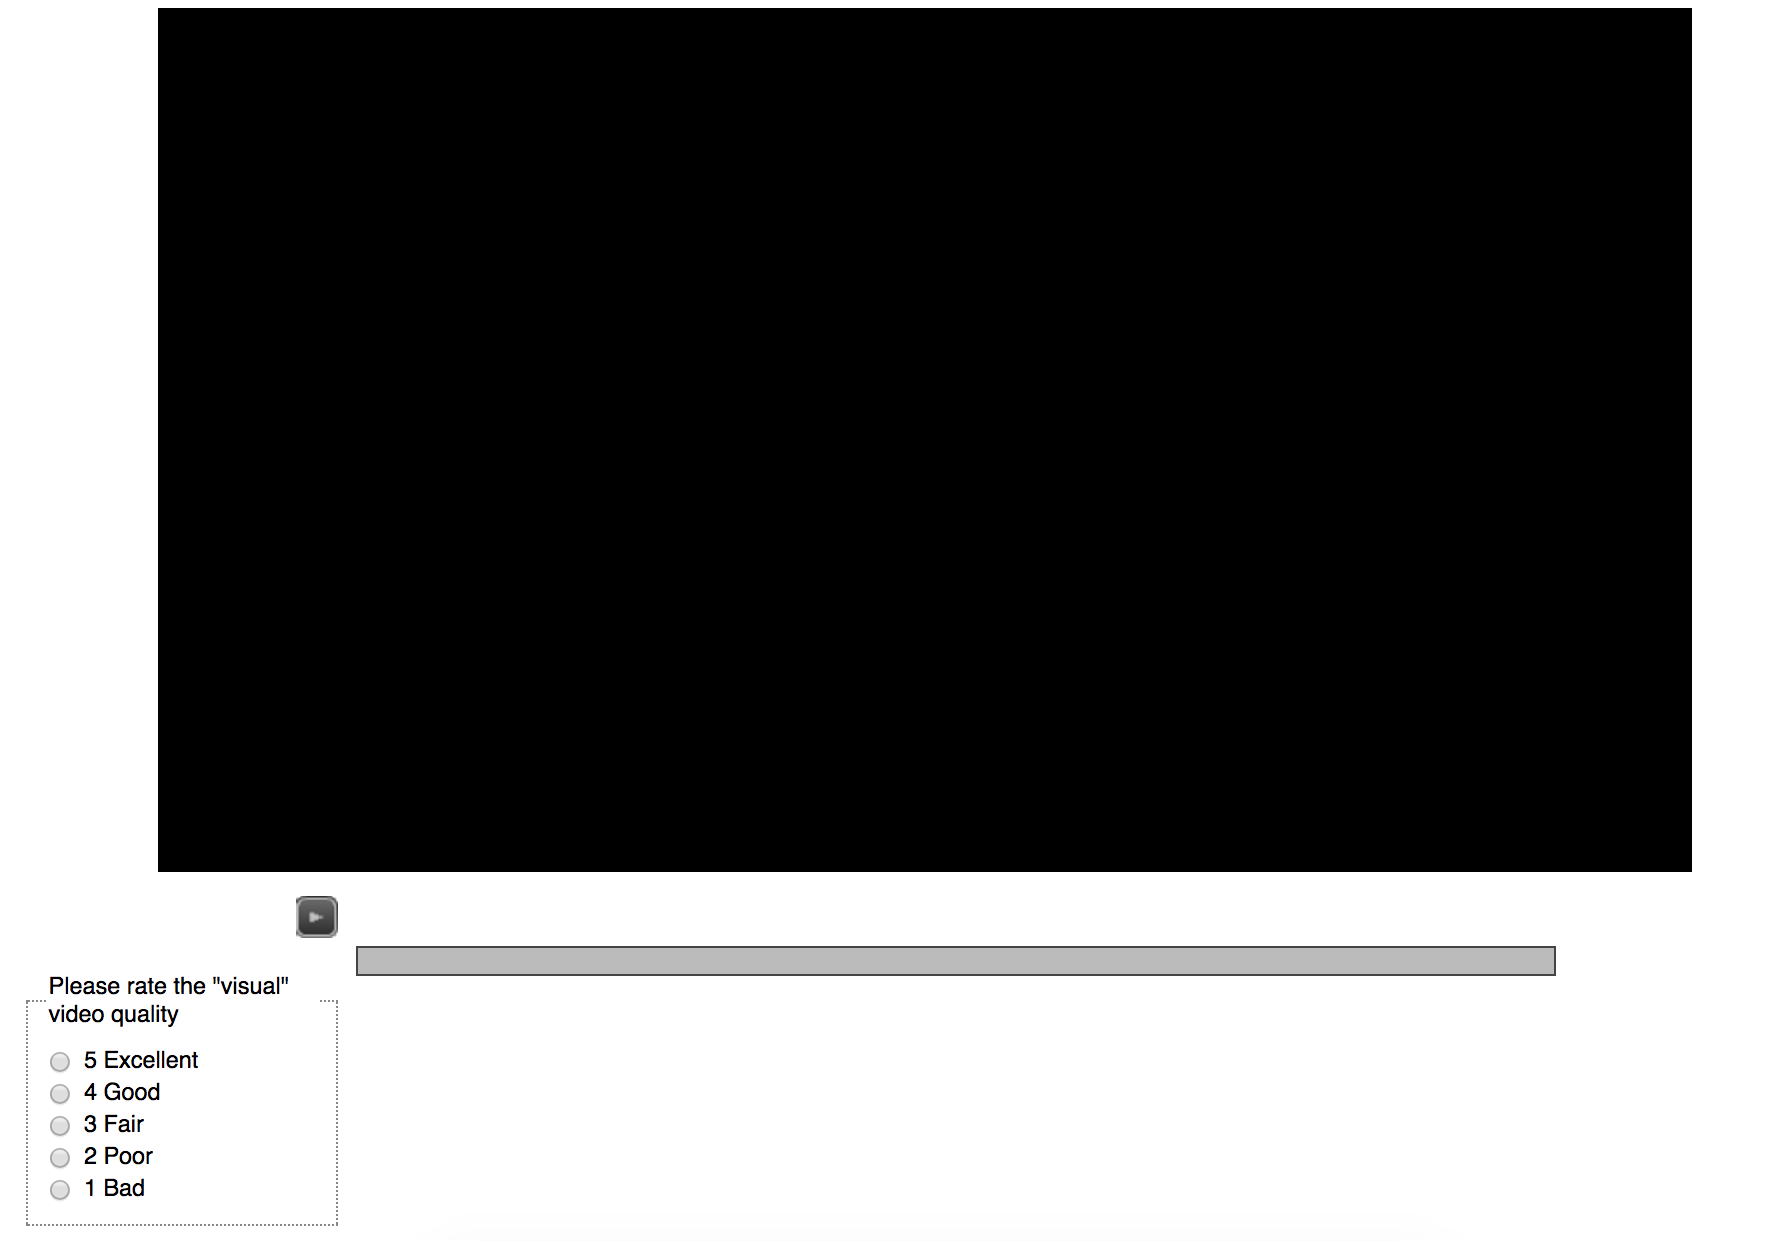
\includegraphics{fig1.png}}
	\end{figure}   
\end{frame}

\begin{frame}
\frametitle{Experimental Design}
	\begin{itemize}
		\item No repetitions of the videos were included. (Time concerns)
		\item Random block included. (To account for possible biases)
		\item No separate voting time (However, cannot click Next before voting)
        \item Crowdsourcing (Test environment)
        %\item No stabilization phase (Time concerns)
	\end{itemize}
\end{frame}

\subsection{Results}
\begin{frame}
   \frametitle{Results}
   \begin{figure}
   		\centering
   		\scalebox{0.5}{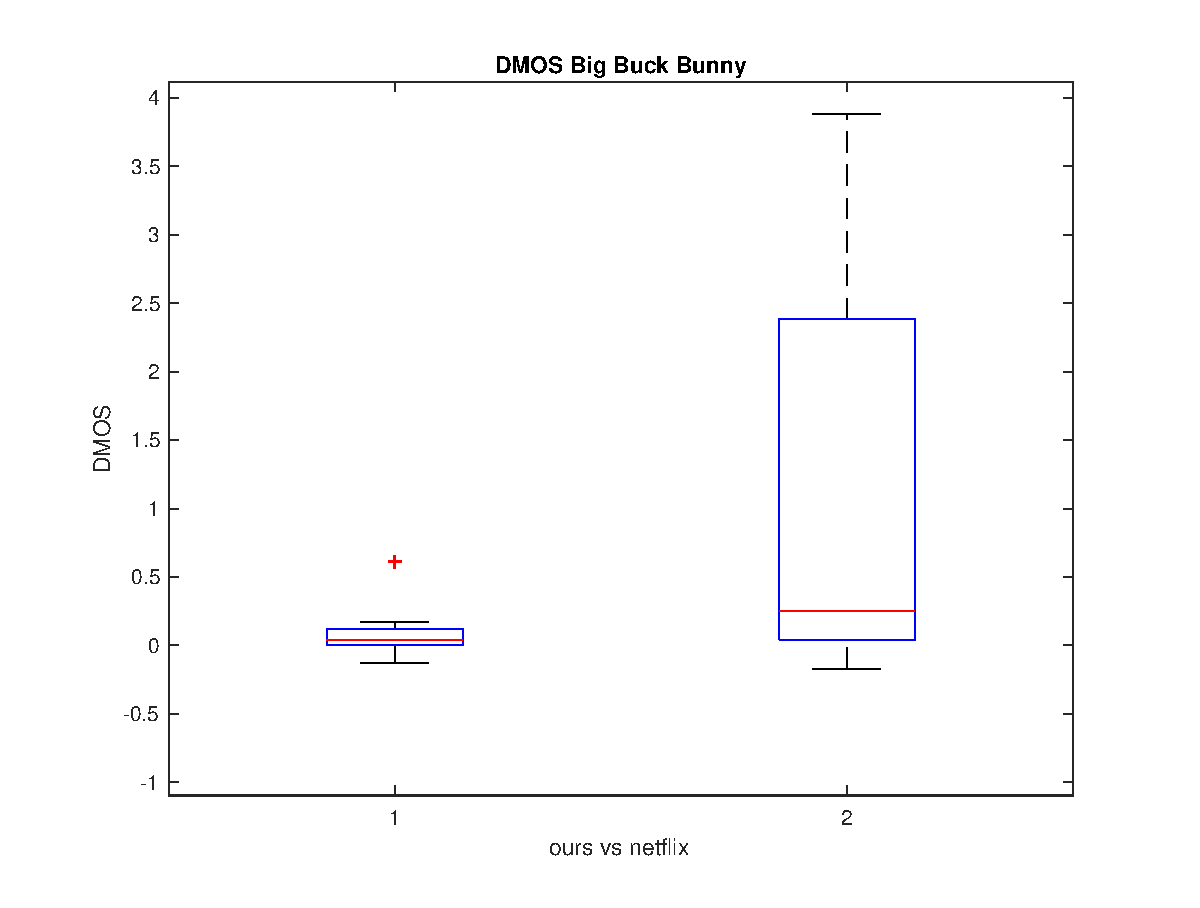
\includegraphics{fig2.eps}}
   \end{figure}
\end{frame}

\begin{frame}
   \frametitle{Results}
   \begin{figure}
   		\centering
   		\scalebox{0.5}{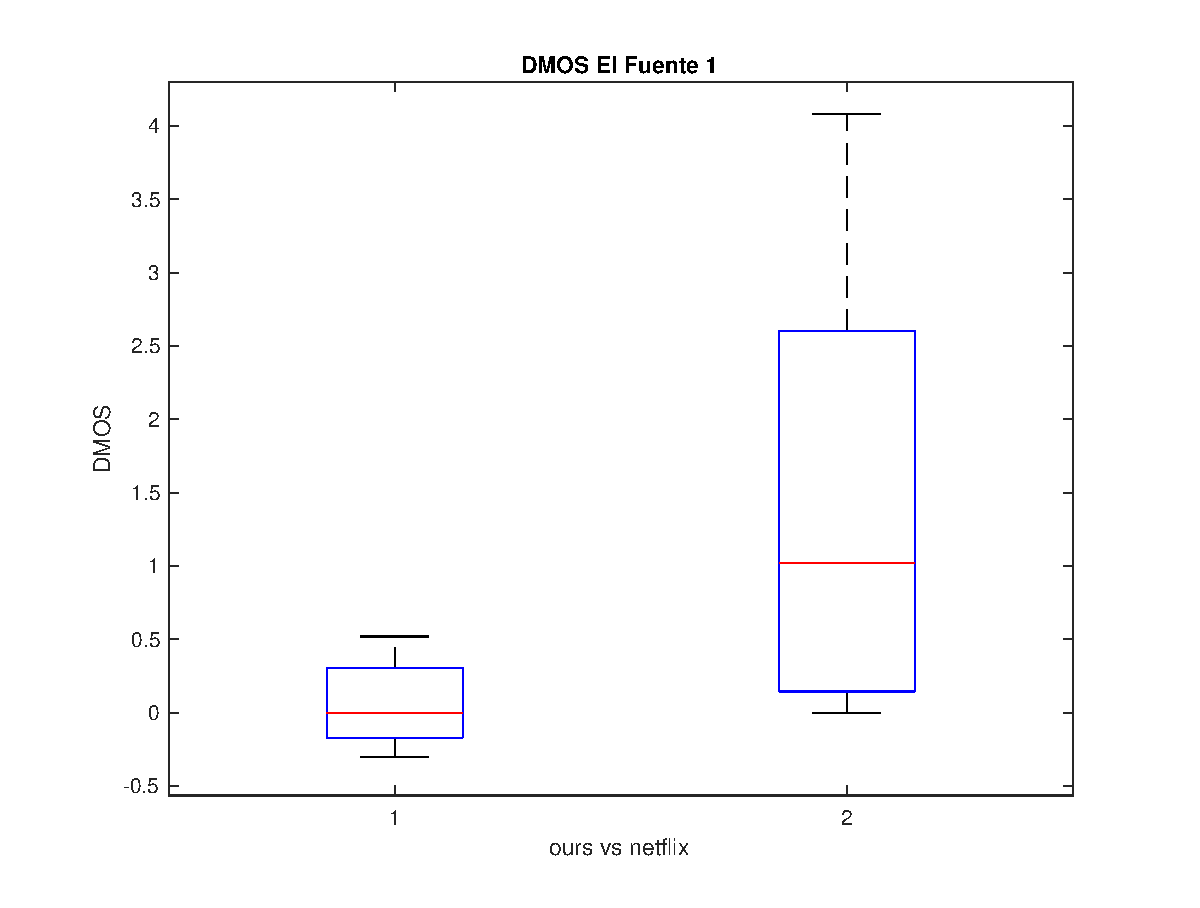
\includegraphics{fig3.eps}}
   \end{figure}
\end{frame}

\begin{frame}
   \frametitle{Results}
   \begin{figure}
   		\centering
   		\scalebox{0.5}{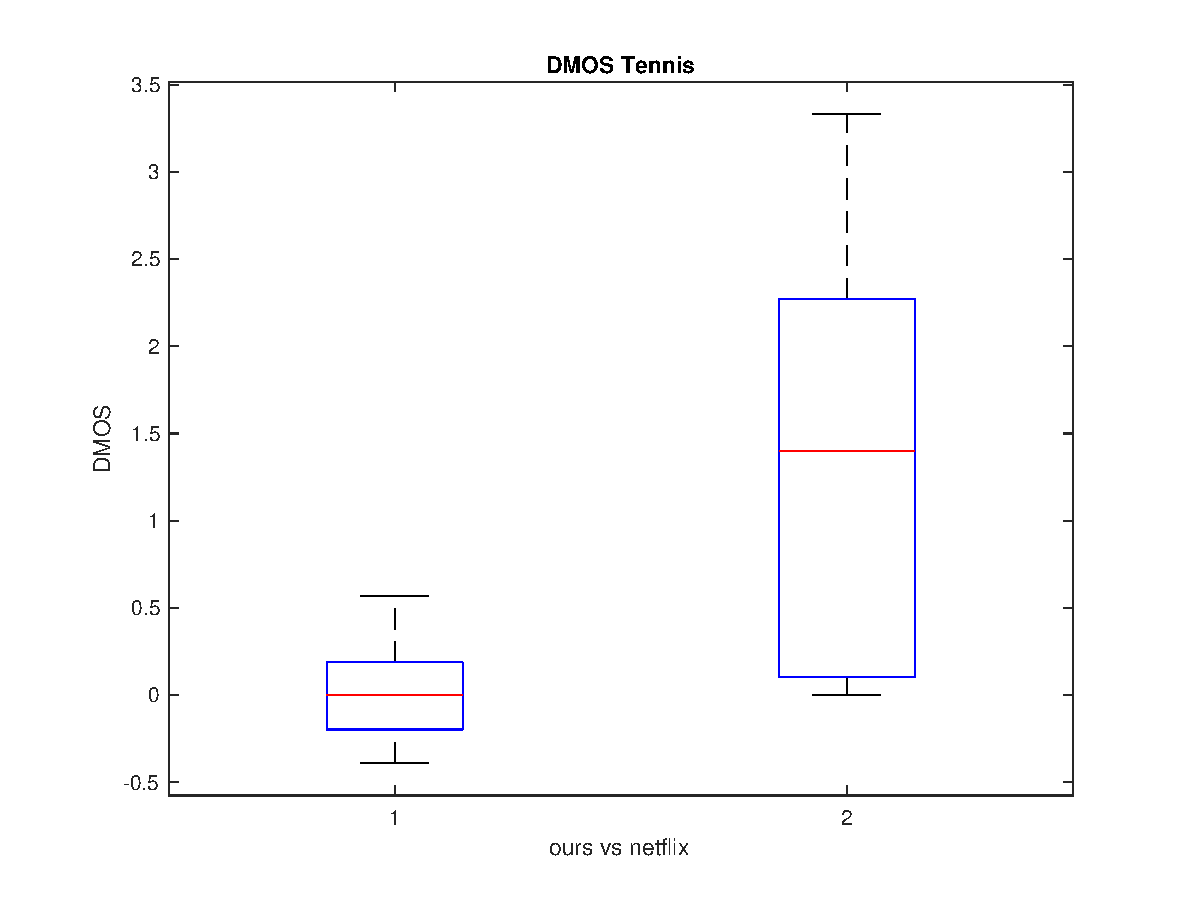
\includegraphics{fig4.eps}}
   \end{figure}
\end{frame}

\begin{frame}
   \frametitle{Results}
   \begin{figure}
   		\centering
   		\scalebox{0.5}{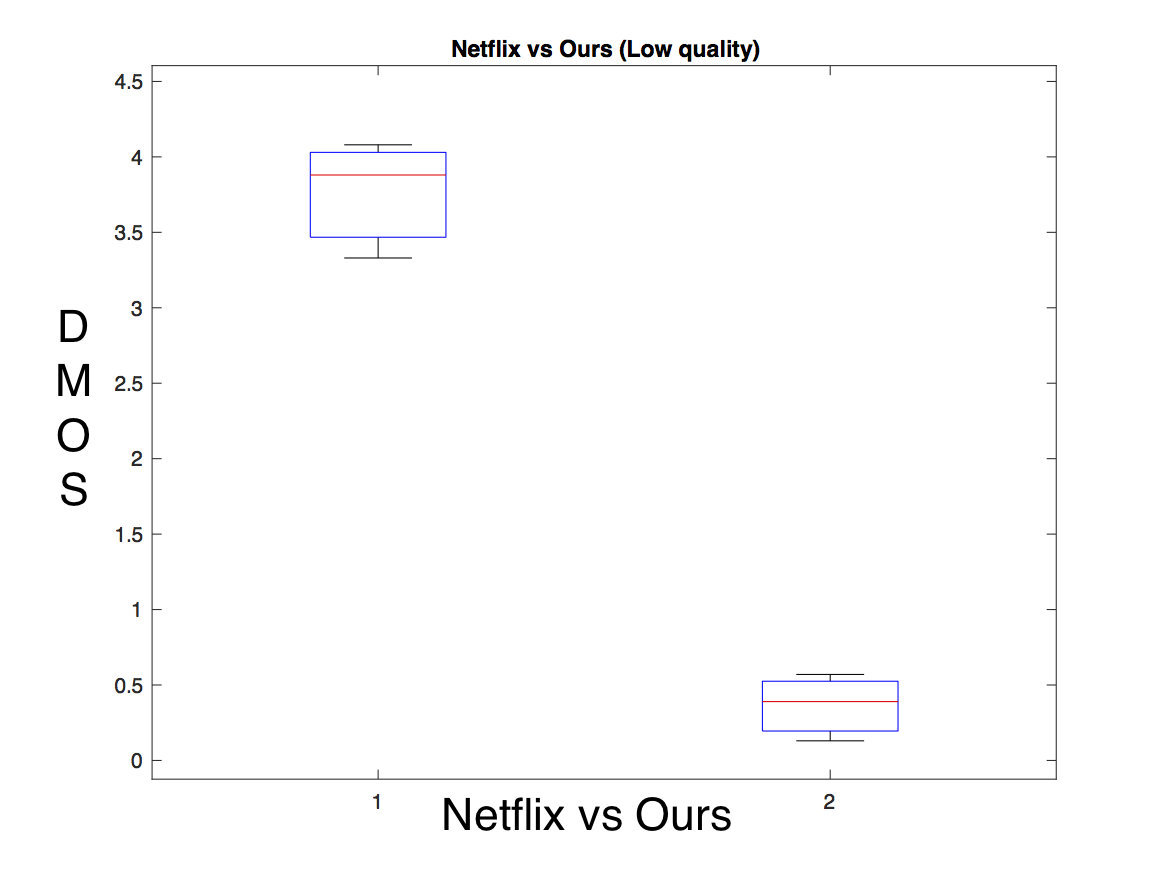
\includegraphics{fig5_.png}}
   \end{figure}
\end{frame}

\begin{frame}
   \frametitle{Results}
   \begin{figure}
   		\centering
   		\scalebox{0.5}{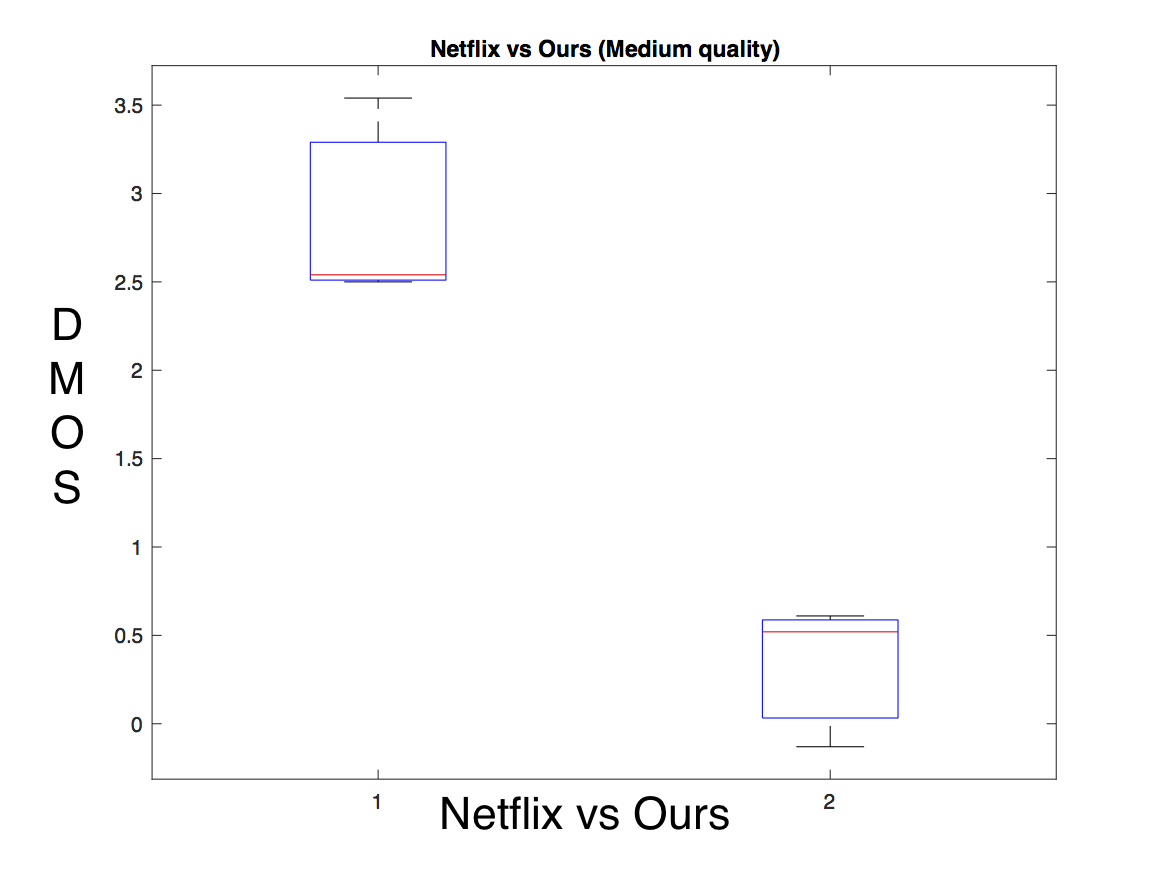
\includegraphics{fig6_.png}}
   \end{figure}
\end{frame}

\begin{frame}
   \frametitle{Results}
   \begin{figure}
   		\centering
   		\scalebox{0.5}{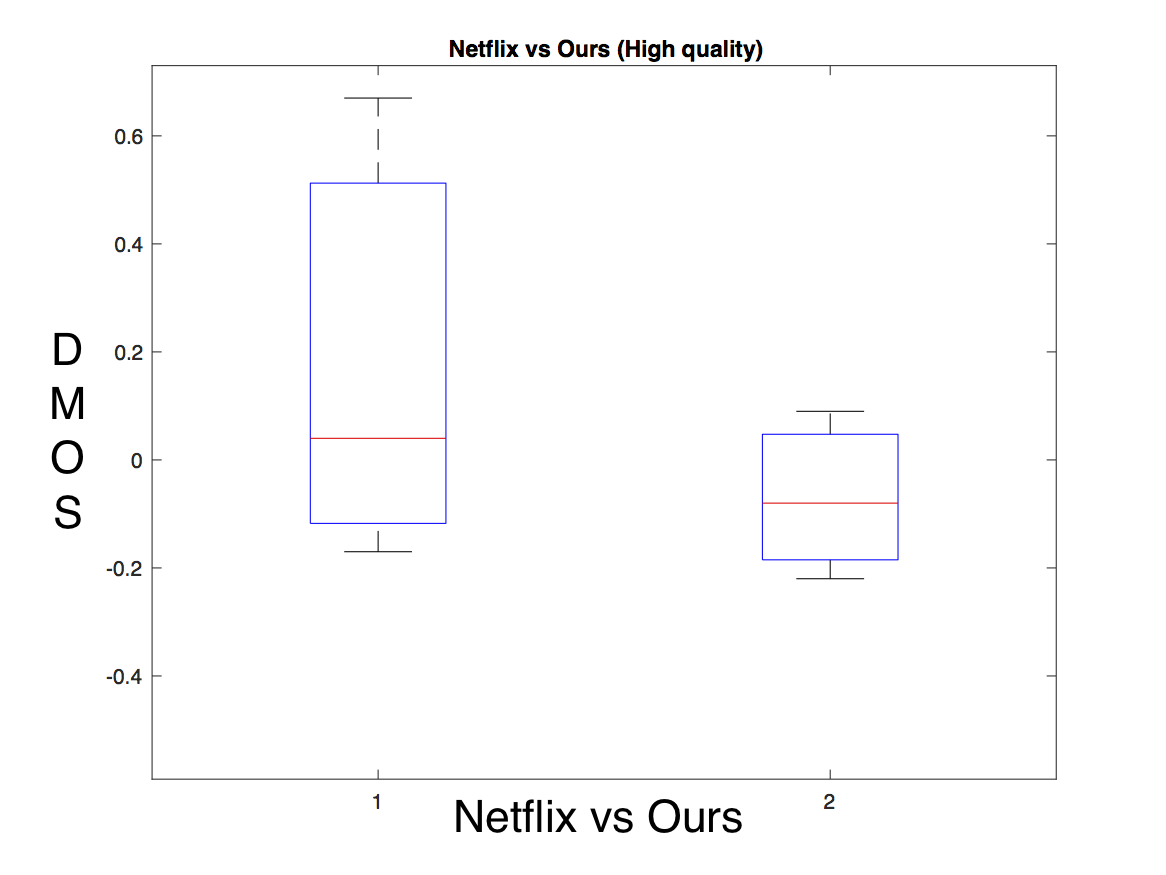
\includegraphics{fig7_.png}}
   \end{figure}
\end{frame}

\begin{frame}
   \frametitle{Results}
   \begin{figure}
   		\centering
   		\scalebox{0.5}{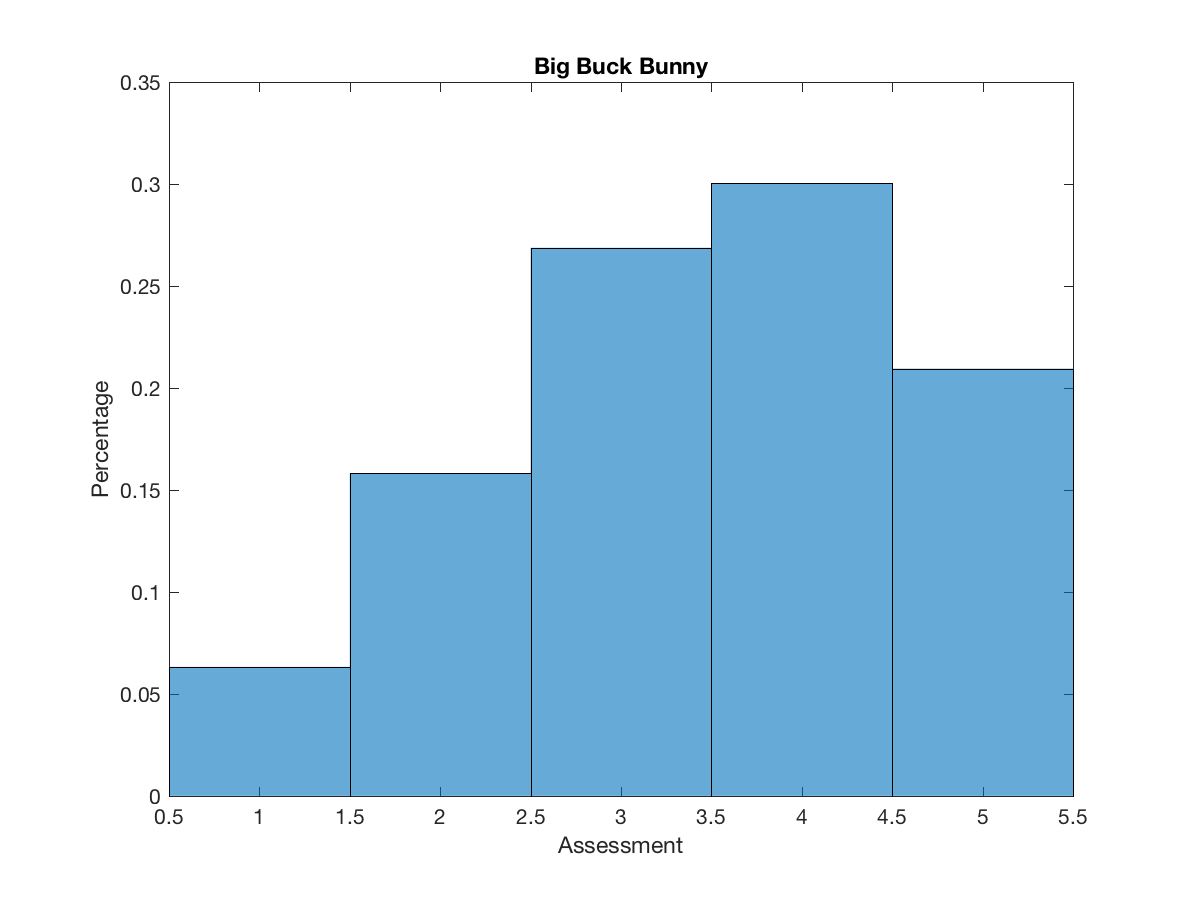
\includegraphics{fig10.eps}}
   \end{figure}
\end{frame}

\begin{frame}
   \frametitle{Results}
   \begin{figure}
   		\centering
   		\scalebox{0.5}{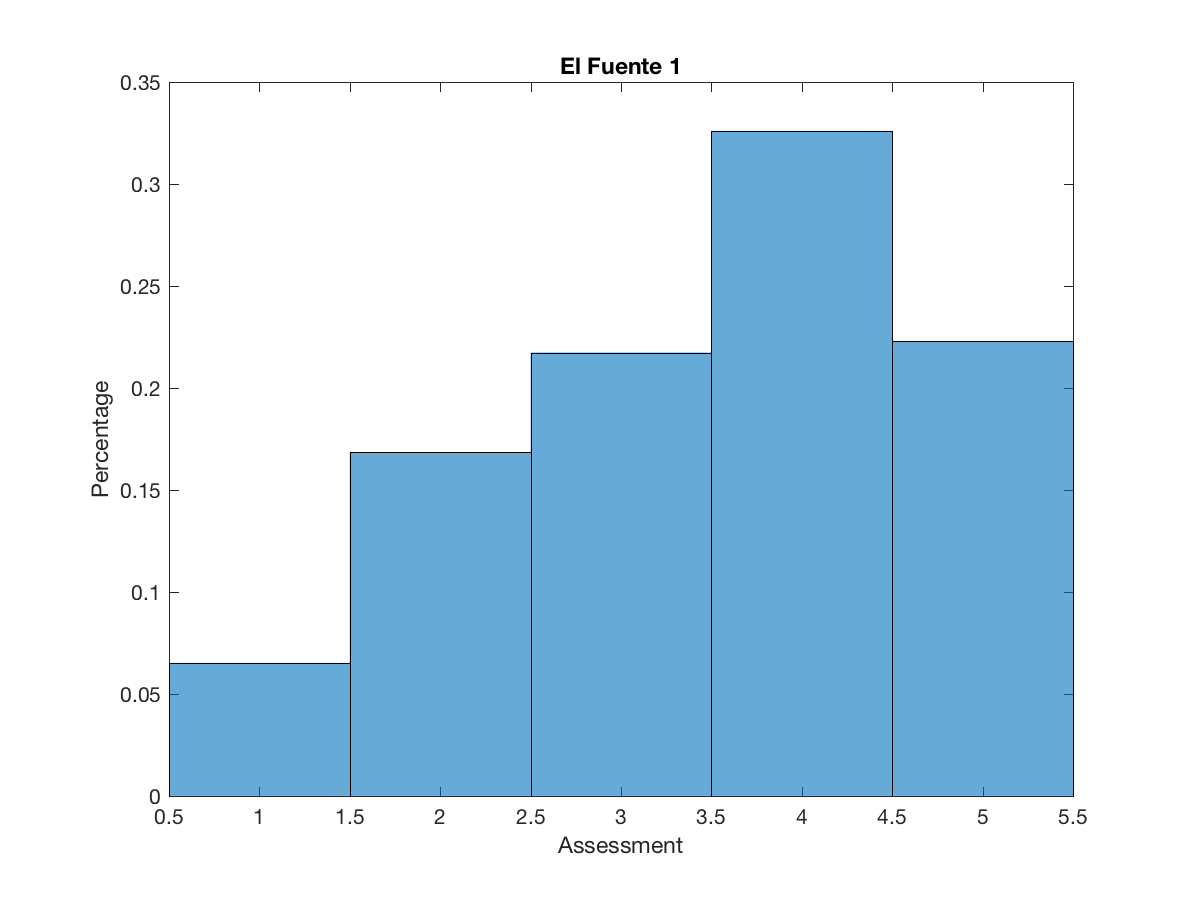
\includegraphics{fig11.eps}}
   \end{figure}
\end{frame}

\begin{frame}
   \frametitle{Results}
   \begin{figure}
   		\centering
   		\scalebox{0.5}{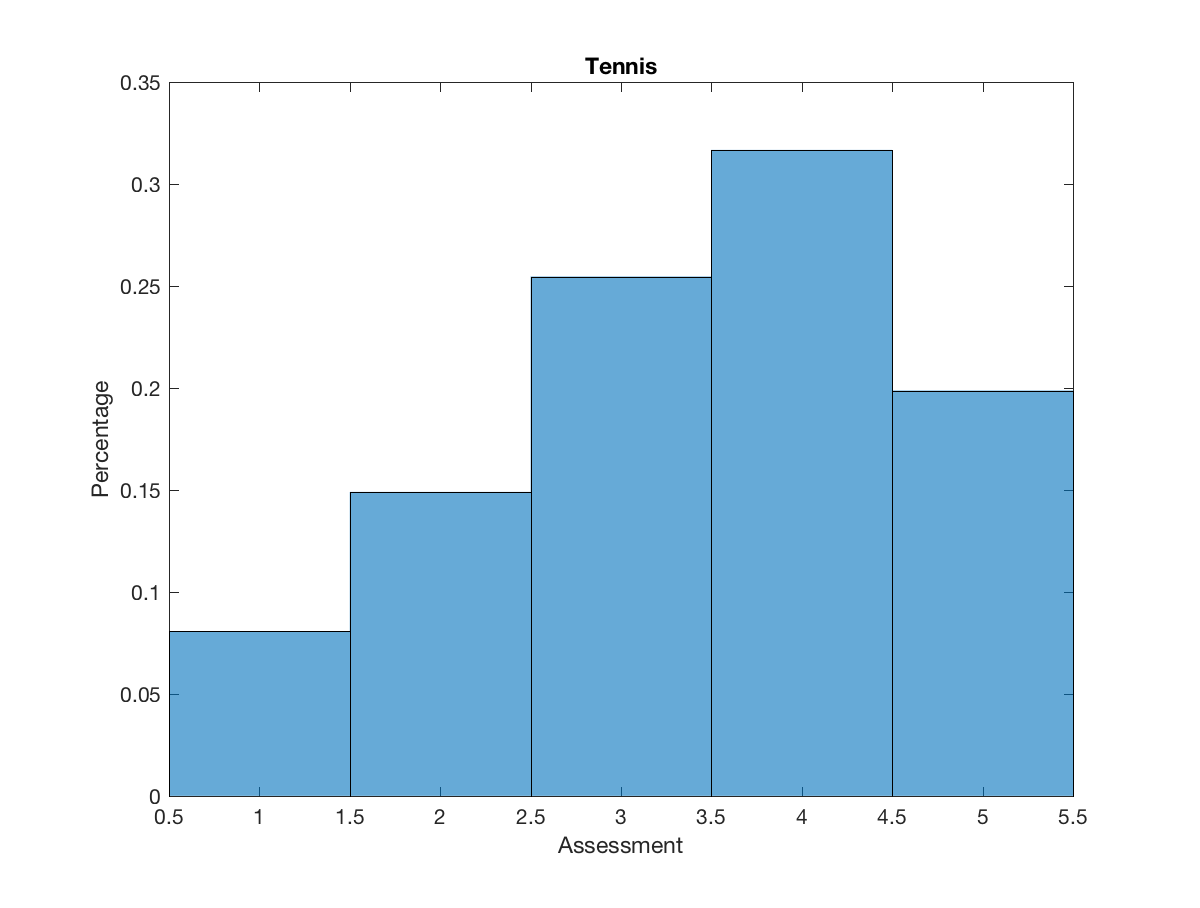
\includegraphics{fig12.eps}}
   \end{figure}
\end{frame}

\begin{frame}
   \frametitle{Results}
   \begin{figure}
   		\centering
   		\scalebox{0.5}{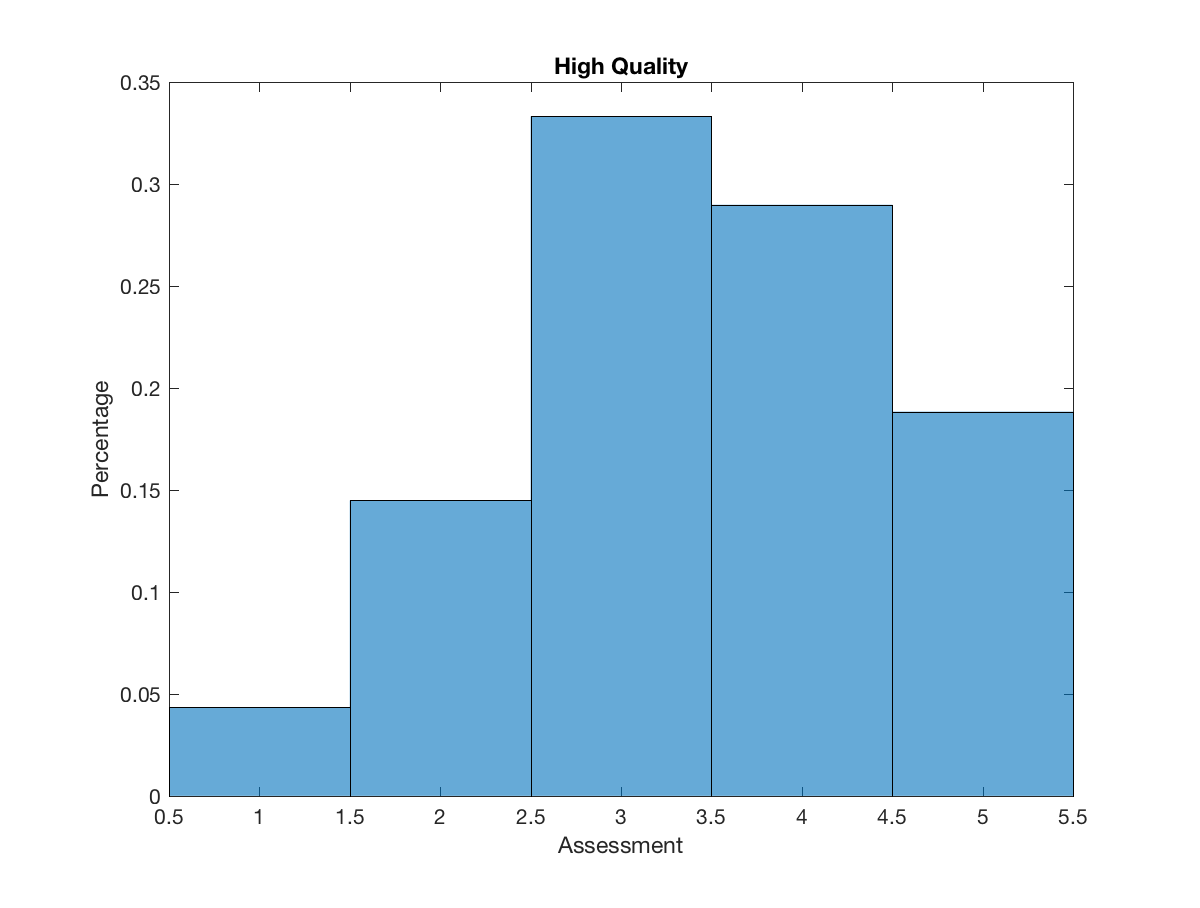
\includegraphics{fig15.eps}}
   \end{figure}
\end{frame}

\begin{frame}
   \frametitle{Results}
   \begin{figure}
   		\centering
   		\scalebox{0.5}{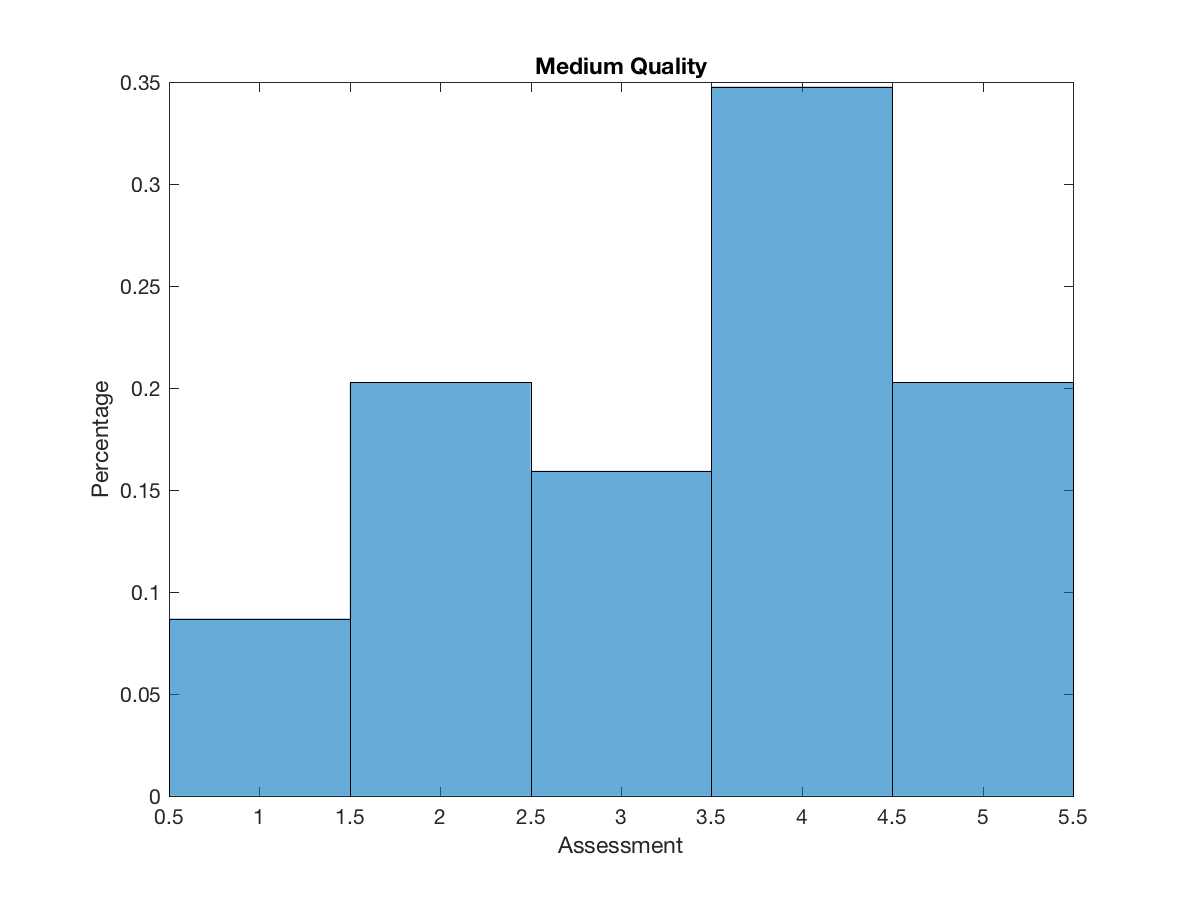
\includegraphics{fig16.eps}}
   \end{figure}
\end{frame}

\begin{frame}
   \frametitle{Results}
   \begin{figure}
   		\centering
   		\scalebox{0.5}{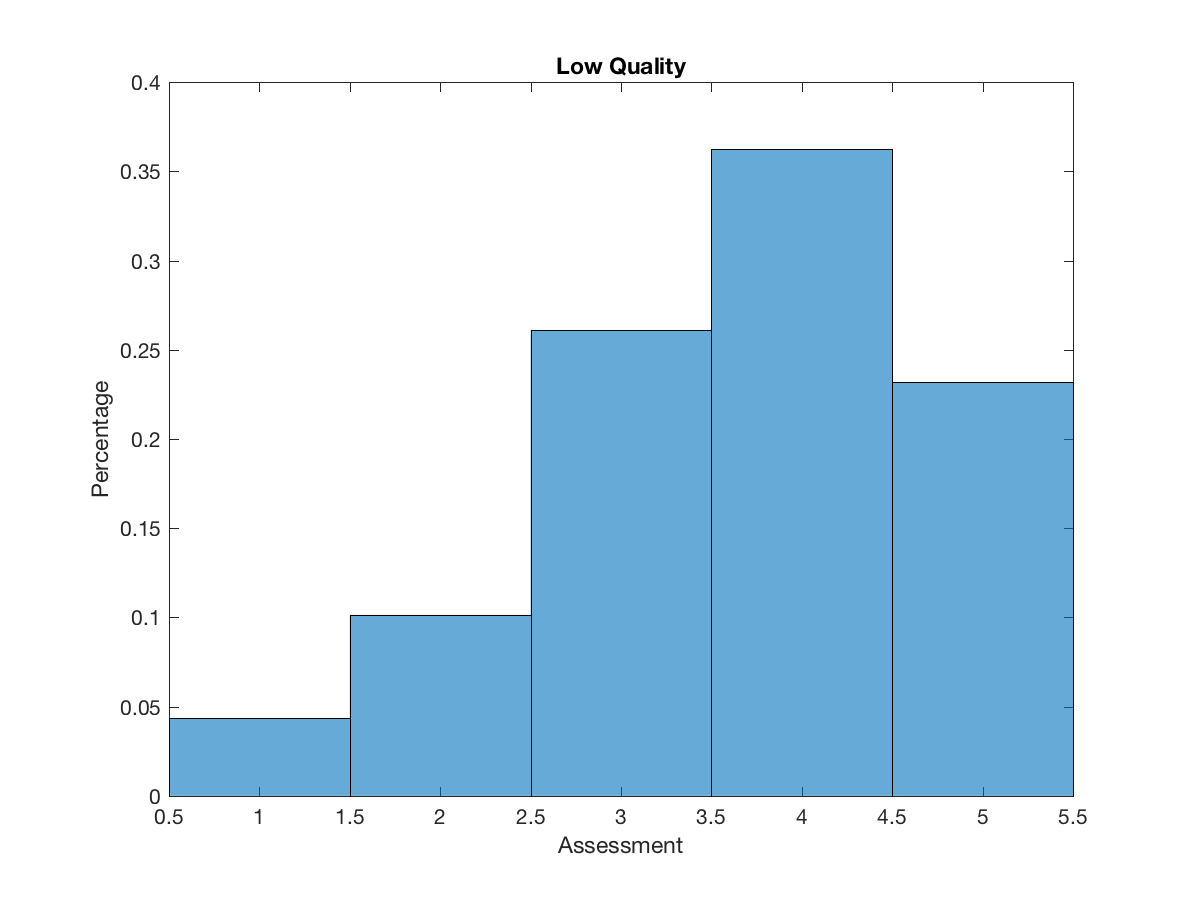
\includegraphics{fig17.eps}}
   \end{figure}
\end{frame}

\begin{frame}
   \frametitle{Subjects}
   \begin{itemize}
      \item From many countries and continents (Germany, Turkey, Italy, etc.)
      \item Mostly friends and family
      \item Average age around 20-25
      \item Mostly men      
     \end{itemize}
\end{frame}



\subsection{Discussion and Conclusion}
\begin{frame}
   \frametitle{Discussion and Conclusion}
   \begin{itemize}
   		\item Random block was not very necessary
   		\item More subjects to take the test
   		\item Many subjects did not finish the test
   		\item Two ends of the scale could have been presented in a better way
   		\item Variation within subjects 
        \item Better outlier detection
   \end{itemize}
\end{frame}

\begin{frame}
	\frametitle{Differences with Netflix}
    \begin{itemize}
    \item Double stimulus impairment scale
    \item 34 source clips / 300 distorted clips
    \item Consumer grade TV, controlled ambient lighting, living room-like environment
    \item No crowdsourcing!
    \item Larger budget!
    \end{itemize}
\end{frame}

\begin{frame}
	\frametitle{Discussion and Conclusion}
    \begin{itemize} 
    	\item Content makes a big difference in assessment (Big Buck Bunny)
    	\item Subjects did not use the full scale
        \item Subjects were generally content with the video quality
    	\item High quality videos as expected
    	\item Surprising results especially in low quality videos
        \item It is difficult to motivate people without incentive
        \item Single stimulus methods are fast, but not reliable
    \end{itemize}
\end{frame}

\section{Video Quality Metric} 
% 2. Part B
\begin{frame}
\frametitle{Part B: Video Quality Metric}
\begin{itemize}
	\item Features Extraction
	\item Models selection
	\item Performance
	\item Discussion and Conclusion
\end{itemize}
\end{frame} 

\begin{frame}
\frametitle{Features Extraction}
\begin{itemize}
	\item \textbf{Features Extracted by Netflix}\itemindent 30pt 
	\item $Vif-scale0,1,2,3...$
    \item Adm2 $(DLM and AIM)$
    \item Motion2
\end{itemize}
\begin{itemize}
    \item \textbf{Features Extracted by ourselves}\itemindent 30pt 
	\item SSIM IW-SSIM MS-SSIM
    \item PSNR
 \end{itemize}    
 \end{frame}

\begin{frame}
\frametitle{SSIM and PSNR}
\begin{itemize}
	\item \textbf{Structural similarity(SSIM)}\itemindent 30pt
    \item Luminance Comparision
    \item Contrast Comparision
    \item Structure Comparision
    \item \(SSIM=l(S,S')c(S,S')s(S,S')\)
\end{itemize}
\begin{itemize}
	\item \textbf{Peak signal-to-noise ratio(PSNR)}\itemindent 30pt
    \item \(PSNR=20log_{10}(MAX_I)-10log_{10}(MSE)\)
\end{itemize}
\begin{itemize}
\item For the YUV video SSIM are:
\item \(SSIM_{ij}=W_YSSIM_{ij}^Y+W_USSIM_{ij}^U+W_VSSIM_{ij}^V\)
\item \(W_Y=0.8 W_U=0.1 W_V=0.1\) 
\end{itemize}

\end{frame}

\begin{frame}
\frametitle{Improved SSIM}
\begin{itemize}
	\item \textbf{Information content weighted structural similarity(IW-SSIM)}
    \item incorporating the idea of information content weighted pooling. 
    \item time costed
\end{itemize}
\begin{itemize}
	\item \textbf{Multi-scale Structural Similarity(MS-SSIM)}
    \item supply more flexibility than single-scale methods in incorporating the variations of image resolution and viewing condition.
    \item Results is similar to the SSIM
\end{itemize}
\end{frame} 


\begin{frame}
\frametitle{Temporal pooling}
\begin{itemize}
	\item Pooling can be done using averaging over all frames 
	\item In this section Mean pooling is better
    \item For other video pooling is a big challenge
\end{itemize}
\end{frame} 

\begin{frame}
\frametitle{Results}
\begin{columns}
\begin{column}{5cm}
\begin{figure}
   		\scalebox{0.3}{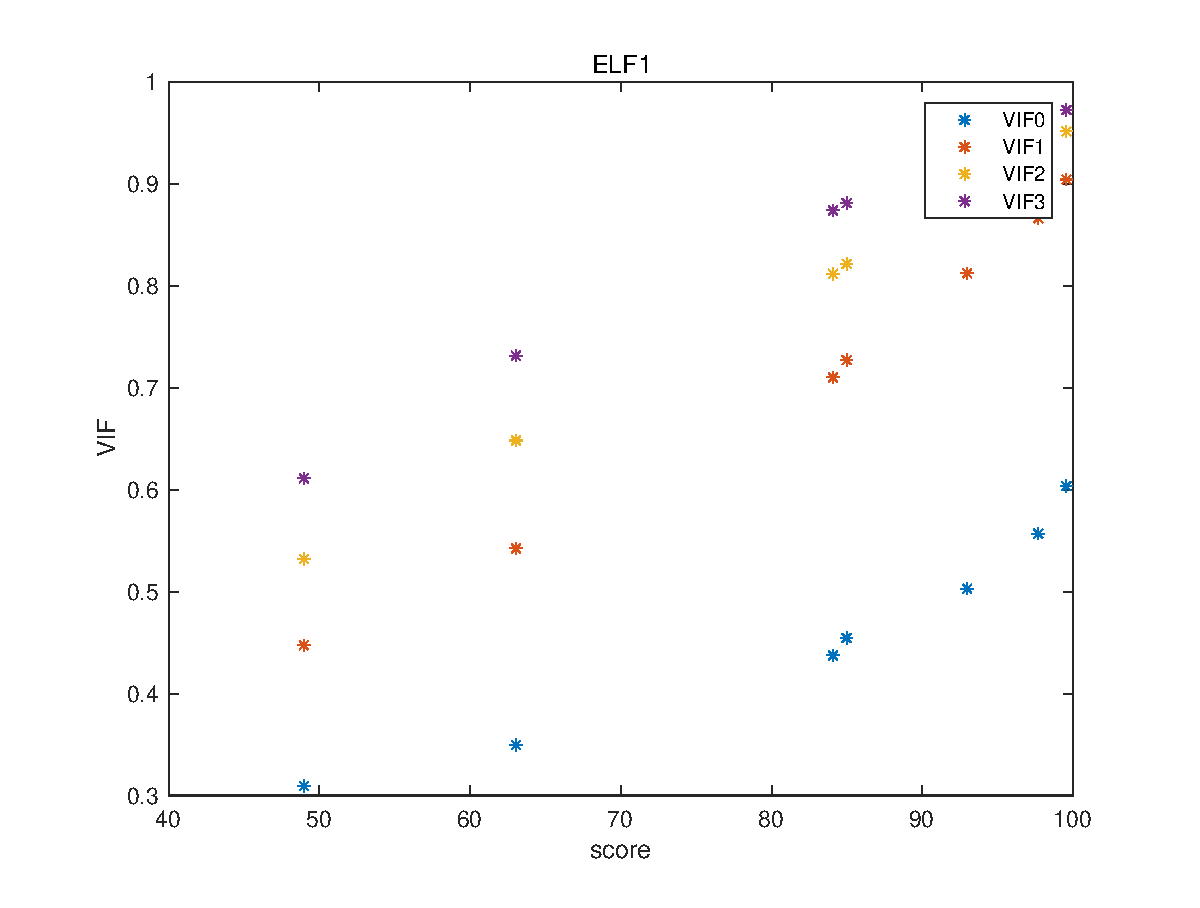
\includegraphics{VIF.eps}}
   \end{figure}
   \end{column}
   \begin{column}{5cm}
\begin{figure}
   		\scalebox{0.3}{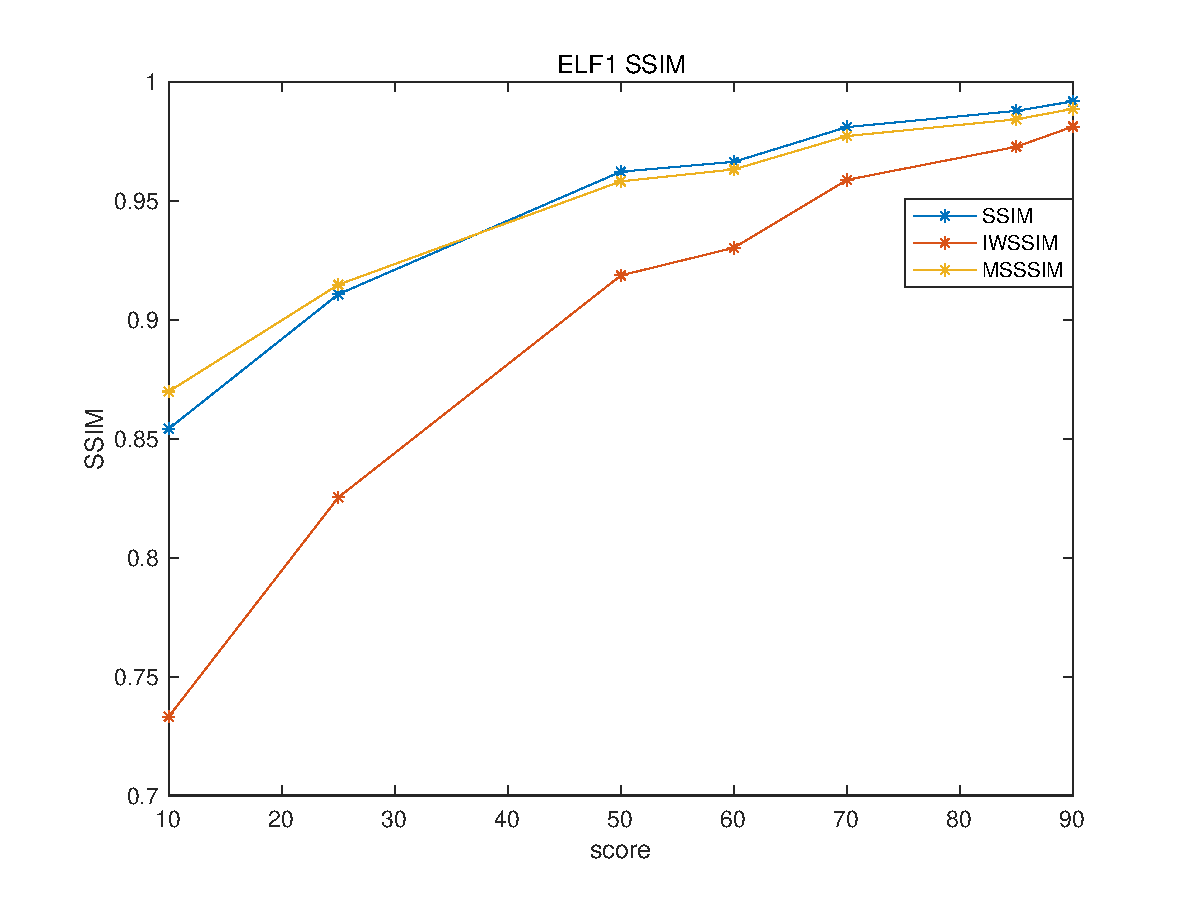
\includegraphics{ELFSSIM.eps}}
   \end{figure}
   \end{column}
   \end{columns}
   
\end{frame} 

\begin{frame}
\frametitle{Regression Models}
	\begin{block}{Principal Components Regression PCR}
		 Only creates components to explain the observed variability in the features
	\end{block}
	\begin{block}{Partial Least Squares Regression PLSR}
		 Also takes the response variable into account, namely the MOS 
	\end{block}
\end{frame} 

\begin{frame}
	\frametitle{Data preprocessing}
	\begin{itemize}
		\item Removal of unreliable subjects:VQEG
	\end{itemize}
	\begin{figure}
		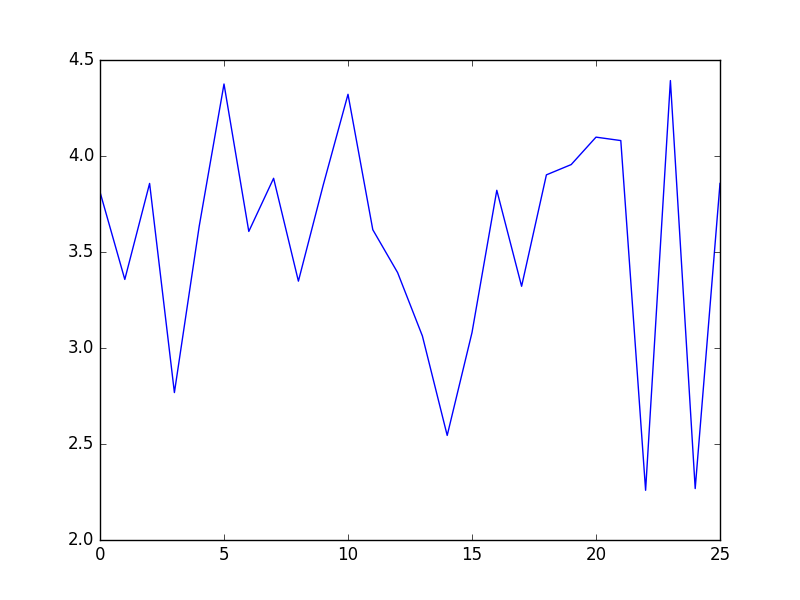
\includegraphics[scale=0.35]{images/crowdsourced_MOS.png} 
		\caption{MOS from Crowdsourcing after 3 Iterations}
	\end{figure}
\end{frame} 

\begin{frame}
\frametitle{Data preprocessing}

	\begin{itemize}
		\item Normalization
	\end{itemize}


 \begin{columns}
		\begin{column}{6cm}
			\begin{figure}
	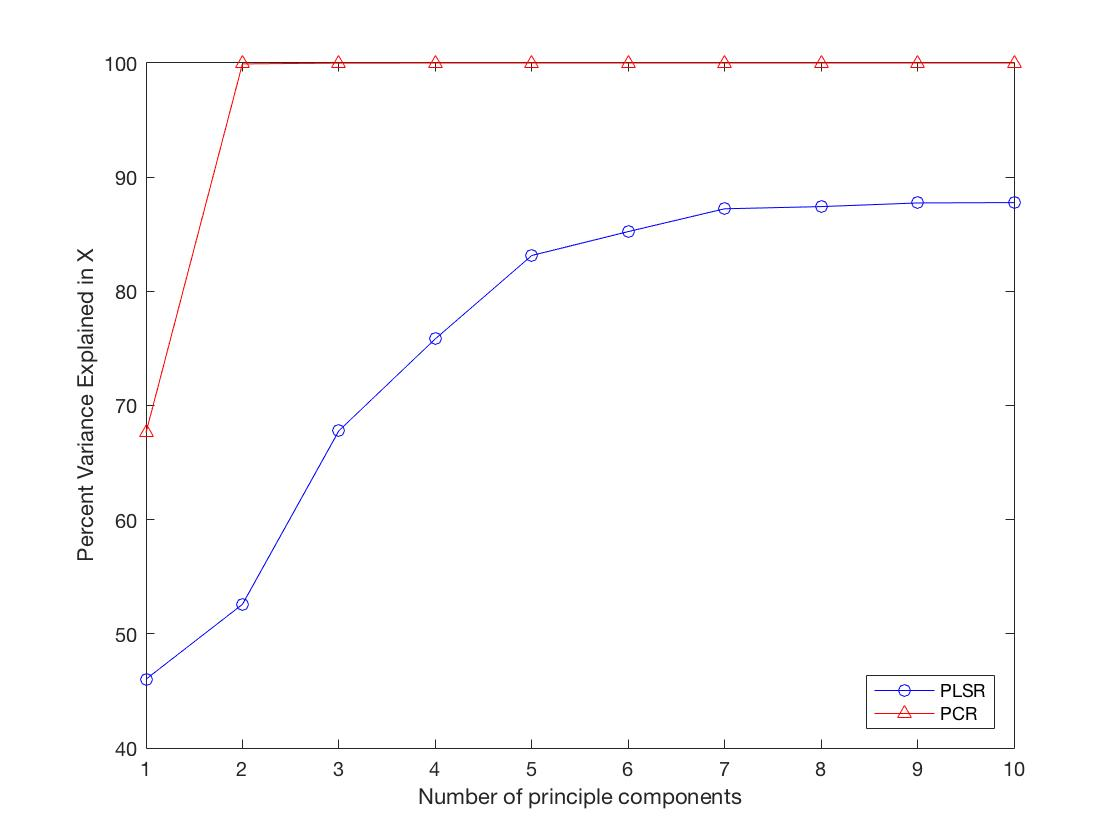
\includegraphics[scale=0.17]{images/PCs+psnr_row} 
	\caption{Percent Variance without normalization}
\end{figure}
		\end{column}
		\begin{column}{6cm}
			\begin{figure}
				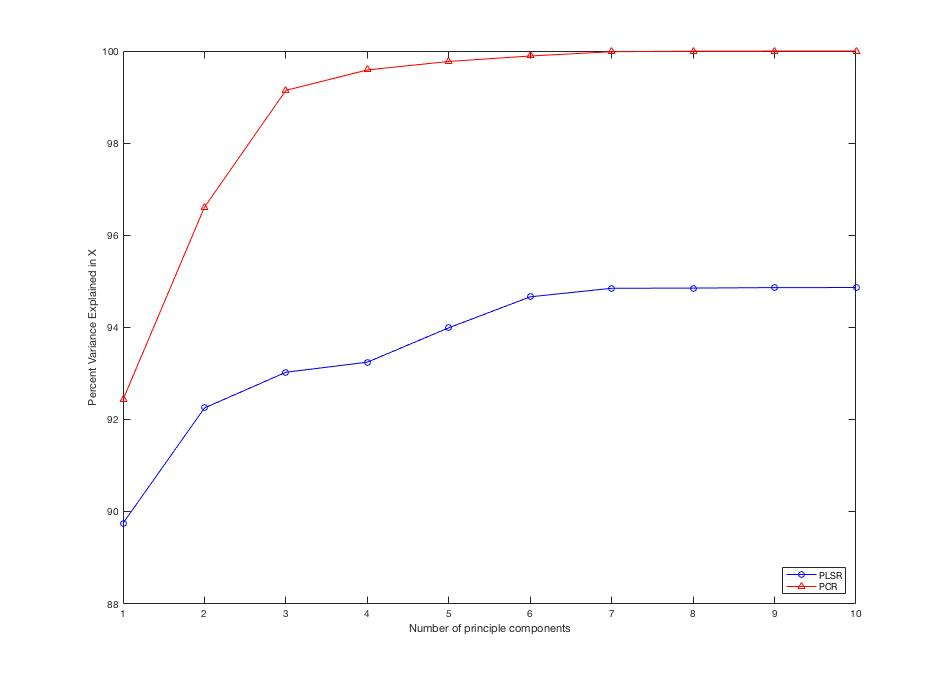
\includegraphics[scale=0.2]{images/PCs+psnr} 
				\caption{Percent Variance + psnr}
			\end{figure}
		\end{column}
	\end{columns}

\end{frame} 

\begin{frame}
\frametitle{Performance}
	\begin{columns}
		\begin{column}{6cm}
			\begin{figure}
				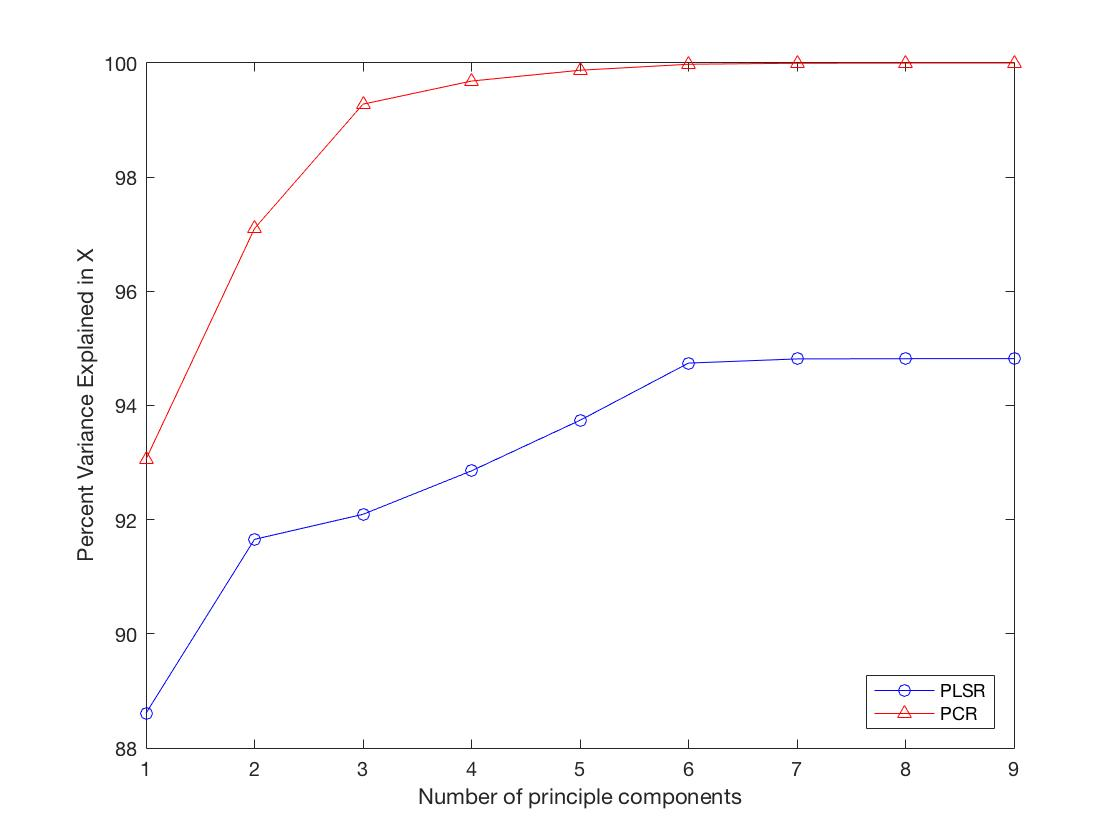
\includegraphics[scale=0.16]{images/PCs} 
				\caption{Percent Variance}
			\end{figure}
		\end{column}
		\begin{column}{6cm}
			\begin{figure}
				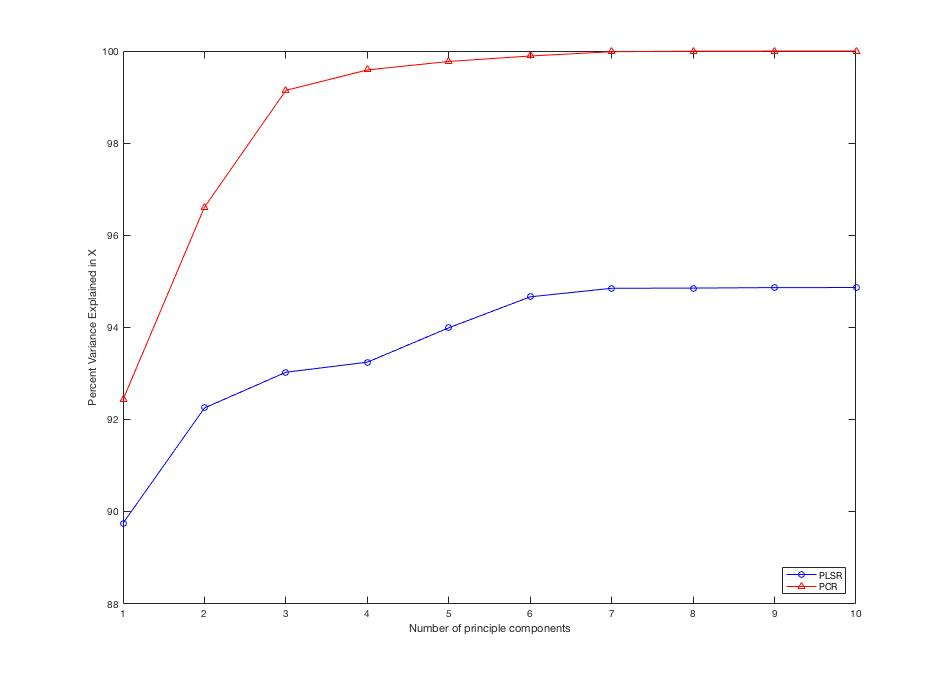
\includegraphics[scale=0.2]{images/PCs+psnr} 
				\caption{Percent Variance + psnr}
			\end{figure}
		\end{column}
	\end{columns}
\end{frame} 

\begin{frame}
\frametitle{Performance}
	\begin{columns}
		\centering
	\begin{column}{6cm}
		\begin{figure}
			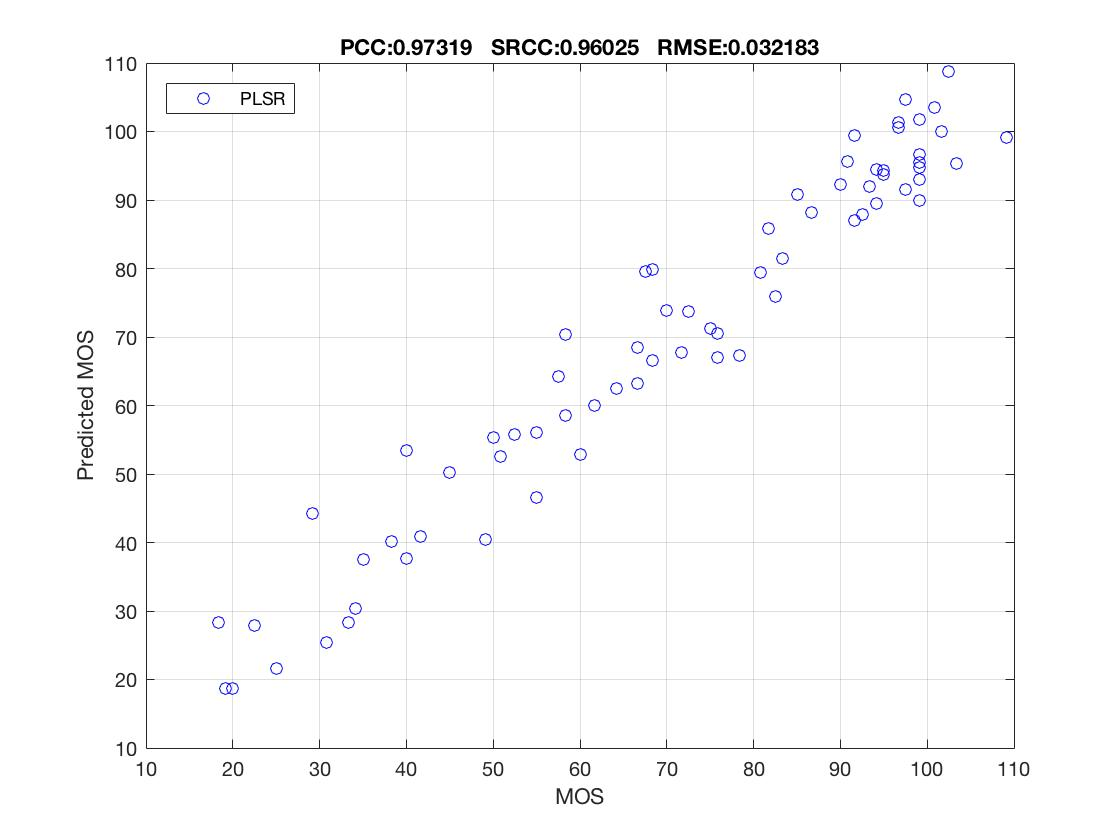
\includegraphics[scale=0.17]{images/PLS_testResult} 
			\centering
			\caption{PLS}
		\end{figure}
	\end{column}
	\centering
	\begin{column}{6cm}
		\begin{figure}
			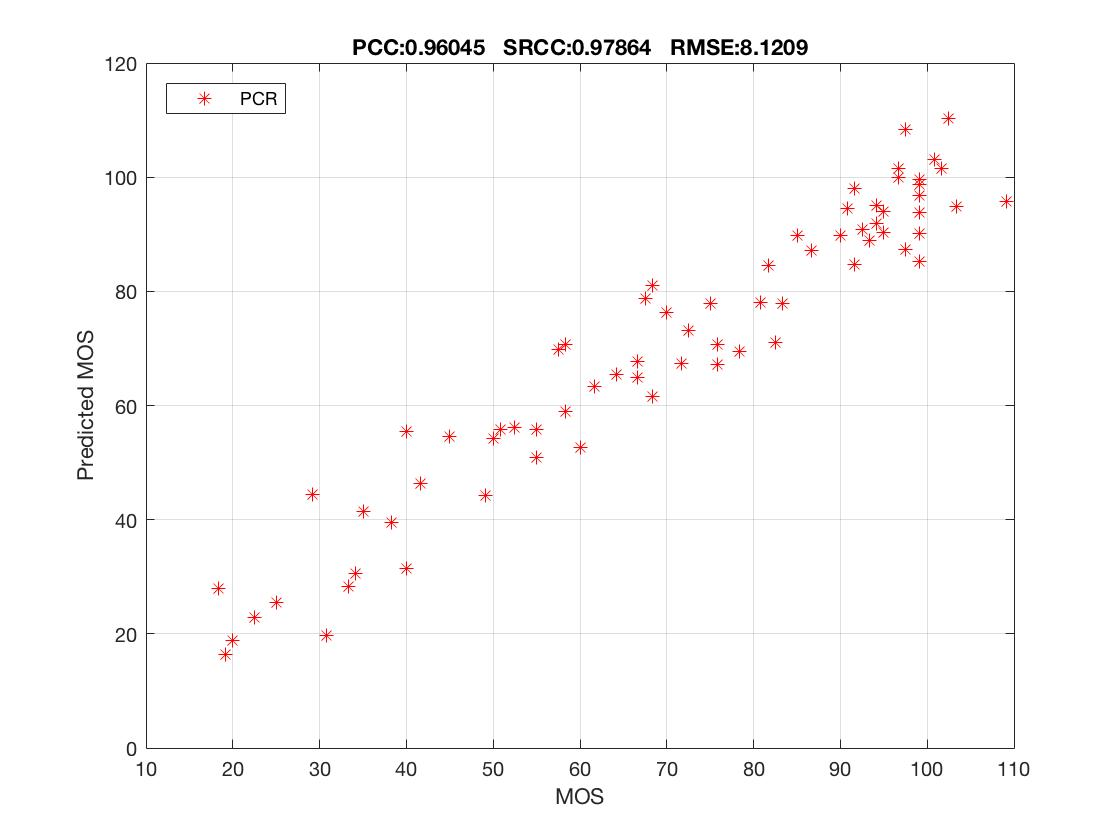
\includegraphics[scale=0.17]{images/PCR_testResult.jpg} 
			\centering
			\caption{PCR}
		\end{figure}
	\end{column}
\end{columns}
\end{frame} 


\begin{frame}
\frametitle{Performance}
\begin{figure}
	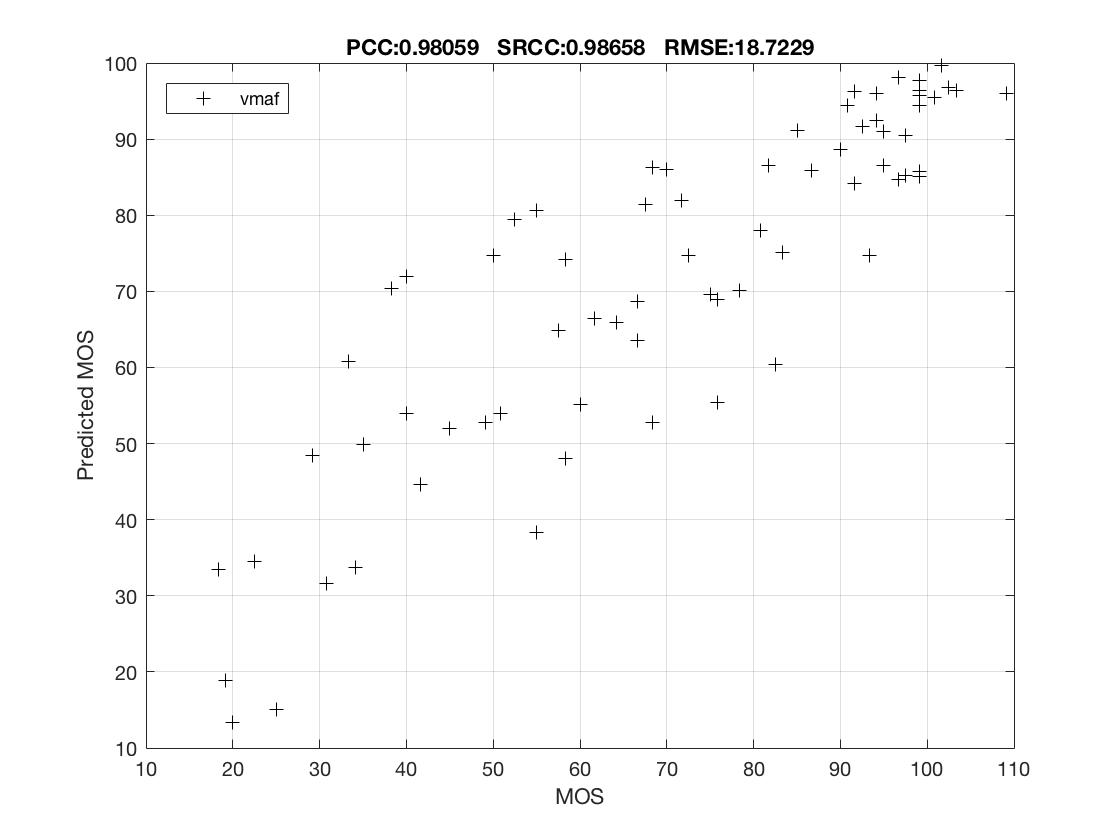
\includegraphics[scale=0.2]{images/vmaf_testResult} 
	\centering
	\caption{vmaf}
\end{figure}
\end{frame} 

\begin{frame}
\frametitle{Performance}
\begin{columns}
	\centering
	\begin{column}{6cm}
		\begin{figure}
			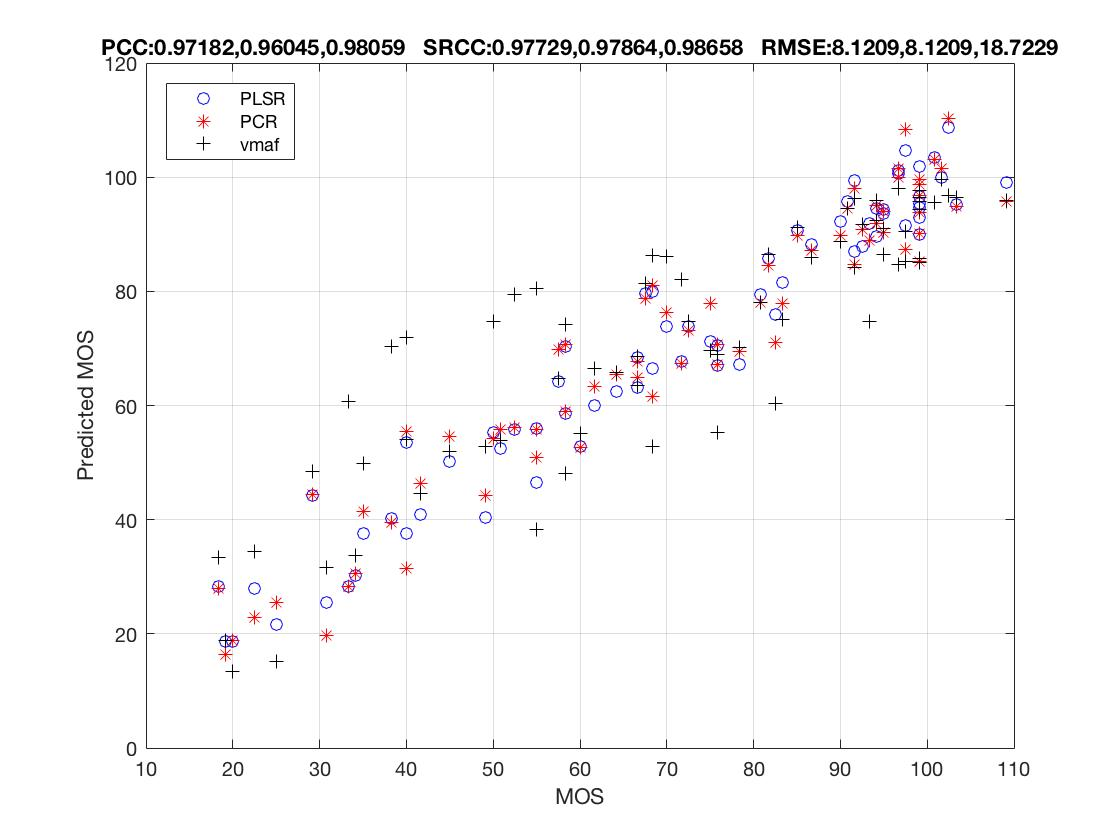
\includegraphics[scale=0.17]{images/all_testResult} 
			\centering
			\caption{all}
		\end{figure}
	\end{column}
	\centering
	\begin{column}{6cm}
		\begin{figure}
			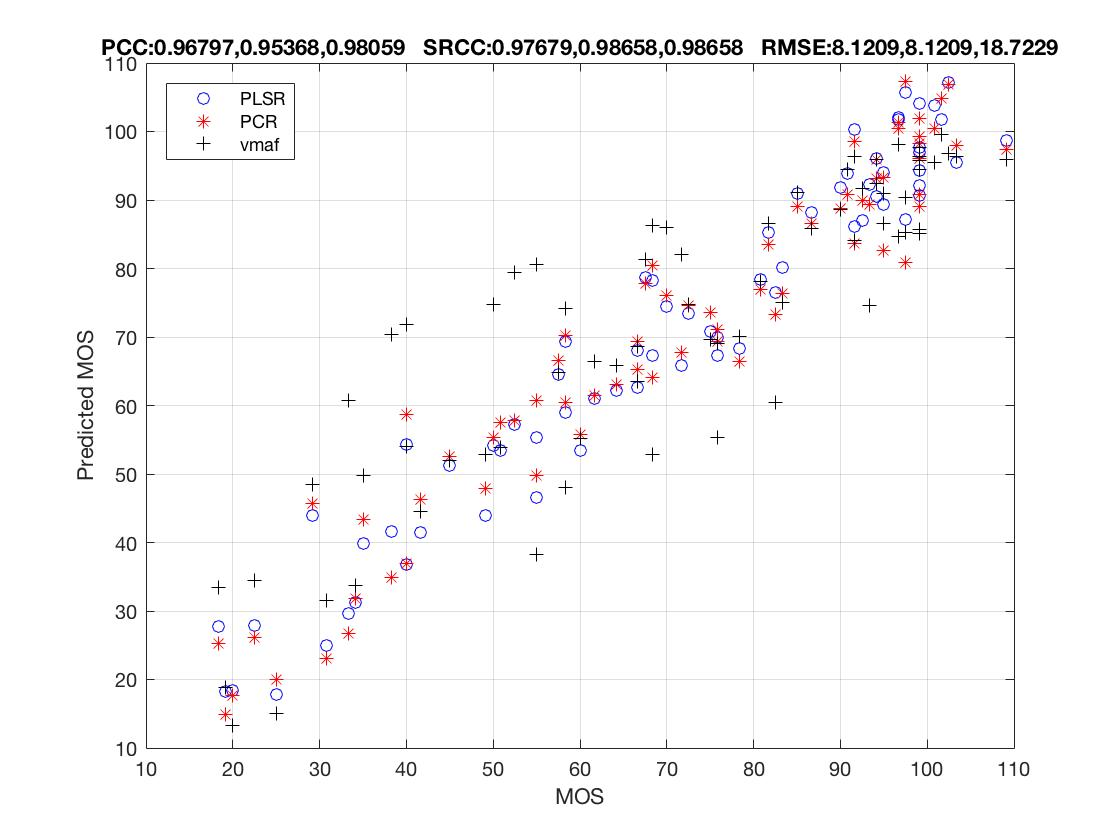
\includegraphics[scale=0.17]{images/all+psnr} 
			\centering
			\caption{all+psnr}
		\end{figure}
	\end{column}
\end{columns}
\end{frame} 

\begin{frame}
\frametitle{Performance}
\begin{table}[!htbp]
	\centering
	\caption{Performance Metrics Of Different Models}
	\label{performance metrics}
	\begin{tabular}{|c|c|c|c|}
		\hline
		\textbf{Models} & \textbf{PCC} & \textbf{SRCC} &\textbf{RMSE}\\
		\hline
		\textbf{PCR(PC=3)} &  0.9550 &  0.9866 & 8.1209  \\
		\hline
		\textbf{PCR(PC=4)} &  0.9599 &  0.9765 & 8.1209  \\
		\hline
		\textbf{PCR(PC=5)} &  0.9554 &  0.9765 & 8.1209 \\
		\hline
		\textbf{PCR(PC=6)} &  0.9605 &  0.9786 & 8.1209  \\
		\hline
		\textbf{PLSR} &  \textbf{0.9718} &  0.9773 & 8.1209   \\
		\hline
		\textbf{PCR+psnr} &  0.9605 &  0.9707 & 8.1209  \\
		\hline
		\textbf{PLSR+psnr} &  0.9717 &  0.9821 & 8.1209  \\
		\hline
		\textbf{VMAF} &  0.9806 &  0.9866 & 18.7229  \\
		\hline
	\end{tabular} 
\end{table}
\end{frame} 

\begin{frame}
\frametitle{Discussion and Conclussion}

\begin{itemize}
	\item Normalization
	\item PLSR performs the best comparing to PCR
	\item Quality of ratings 
	\item Feature selection
\end{itemize}


\end{frame} 
% End Slides
\end{document}



 %End Slides

\end{document}
